\section{Caracterización de los procedimientos simulados}

En esta sección, se describirán los conceptos básicos necesarios para que el lector pueda entender el contexto en el que fueron desarrollado los simuladores que forman parte de los casos de uso para esta tesis. Se describirán los procedimientos médicos tanto de la anestesia regional como de las proyecciones utilizadas en radiología diagnóstica.

\subsection{Anestesia regional}
\label{art:ra}
%\todo{ es importante que describas la RA y la Radiología diagnostica en el estado del arte. Deben ir los pasos detallados del procedimiento. Pon alguna cita en el estado del arte. Por ejemplo, el CV de RA de Cork. Esto luego lo usaras en el courseware}

%\todo{Repite brevemente en que consiste la RA antes de hablar del guiado. Vetajas de este procedimiento y un cita a algún sitio donde describan el procedimiento o documento de rasiams.  }

La \ac{RA} consiste en bloquear un nervio administrando un anestésico local en sus proximidades. Para la localización del nervio objetivo y guiar la aguja, actualmente se utilizan dos técnicas \cite{ded2.1}: el guiado por estimulación eléctrica del nervio (fig. \ref{fig:electrical}) y el uso del ecógrafo (fig. \ref{fig:raus}).

%La \acl{RA}(\acs{RA}) guiada por \acl{US}(\acs{US}) representa una alternativa al guiado por estimulación eléctrica.
Tradicionalmente, el médico encontraba el nervio a través de la administración de una corriente continua sin visualizar la anatomía. Utilizar una imagen de \ac{US} ofrece la ventaja de guiar la aguja a través de todas las estructuras internas como fascias, pleura y vasos sanguíneos. También evita introducir el anestésico en el torrente sanguíneo o dañar el tejido nervioso. Además, es posible confirmar la propagación del anestésico alrededor del nervio objetivo.  

% \begin{figure}[h]
%   \centering
%     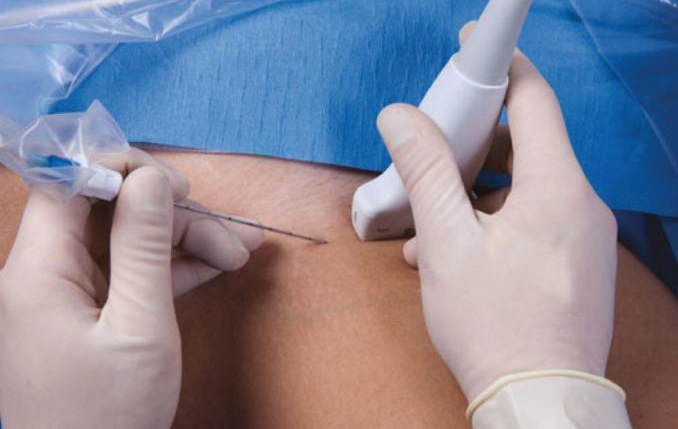
\includegraphics[width=0.5\textwidth]{IMG/RAUS.png}
%     \caption{ Anestesia regional guiada por \acl{US}.}
%   \label{fig:raus}
% \end{figure}
\begin{figure}[h]
   \begin{subfigure}[b]{0.45\linewidth}
        \centering
        {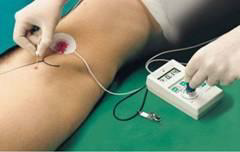
\includegraphics[width=\linewidth]{IMG/electrical.png}}
        \caption{\label{fig:electrical}Anestesia regional guiada por estimulación eléctrica.}
    \end{subfigure}
    \null\hfill
     \begin{subfigure}[b]{0.45\linewidth}
        \centering
        {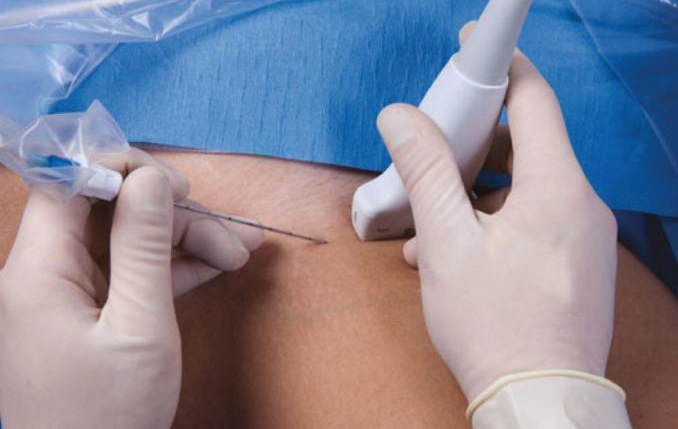
\includegraphics[width=\linewidth]{IMG/RAUS.png}}
        \caption{\label{fig:raus}Anestesia regional guiada por \acl{US}.}
    \end{subfigure}
     
    \caption{Técnicas de \acl{RA}}
   \end{figure}
   
   
Según la zona anatómica donde se realice, la posición del paciente varía y, por tanto, es importante que el médico deba conocer la disposición del nervio a bloquear. Por ejemplo, el bloqueo femoral es probablemente el bloqueo de extremidad inferior que se realiza con más frecuencia por su facilidad y su alta tasa éxito. En este procedimiento, el paciente se coloca decúbito supino. Sin embargo, en el bloqueo axilar, es necesario que el paciente esté en posición de flexión del brazo por contracción del bíceps.

%\todo{Da más datos bloque del nervio femoral ... }

La ejecución de este procedimiento no es sencillo para aquellos profesionales de anestesiología que no están familiarizados con las técnicas de \ac{US}. Además de los conocimientos teóricos, los profesionales deben entrenar sus habilidades no cognitivas. Estos entrenamientos habitualmente se practican con paciente reales, con la utilización de cadáveres \cite{Tsui2007} o el uso de \emph{fantomas} \cite{phantomra}. La incorporación de un simulador en el entrenamiento del procedimiento ayudará a solventar las limitaciones de los entrenamientos clásicos al ser repetible y seguro.


Según el Entregable 2.1 de \ac{RASimAs} titulado \emph{User Specifications} \cite{ded2.1}, el procedimiento de \ac{RA} guiado por \ac{US} se puede separar en los siguientes bloques:
\begin{enumerate}
    \item Exploración (\emph{Scout Scan}): el profesional configura y explora con la sonda de \ac{US} la zona del paciente con el objetivo de identificar el nervio, vasos sanguíneos cercanos y las demás estructuras anatómicas importantes (figura \ref{fig:scoutscan}). 

%\todo{ Las imágenes se ven fatal, las paso a word, word a pdf y las pongo en el anexo? puedo citarlas también en los resultados}
    \item Guiado de la aguja (\emph{Needle Guidance}): cuando el profesional está seguro de haber interpretado la imagen de \ac{US}, guía la aguja a través de la anatomía hasta aproximarse al nervio (figura \ref{fig:needleguidance}).  
   
    \item Inyección (\emph{Injection}): el médico libera el bolo y confirma que se ha realizado correctamente el bloqueo del nervio (figura \ref{fig:injection}). 
   
\end{enumerate}
\begin{figure}[bh]
  \centering
    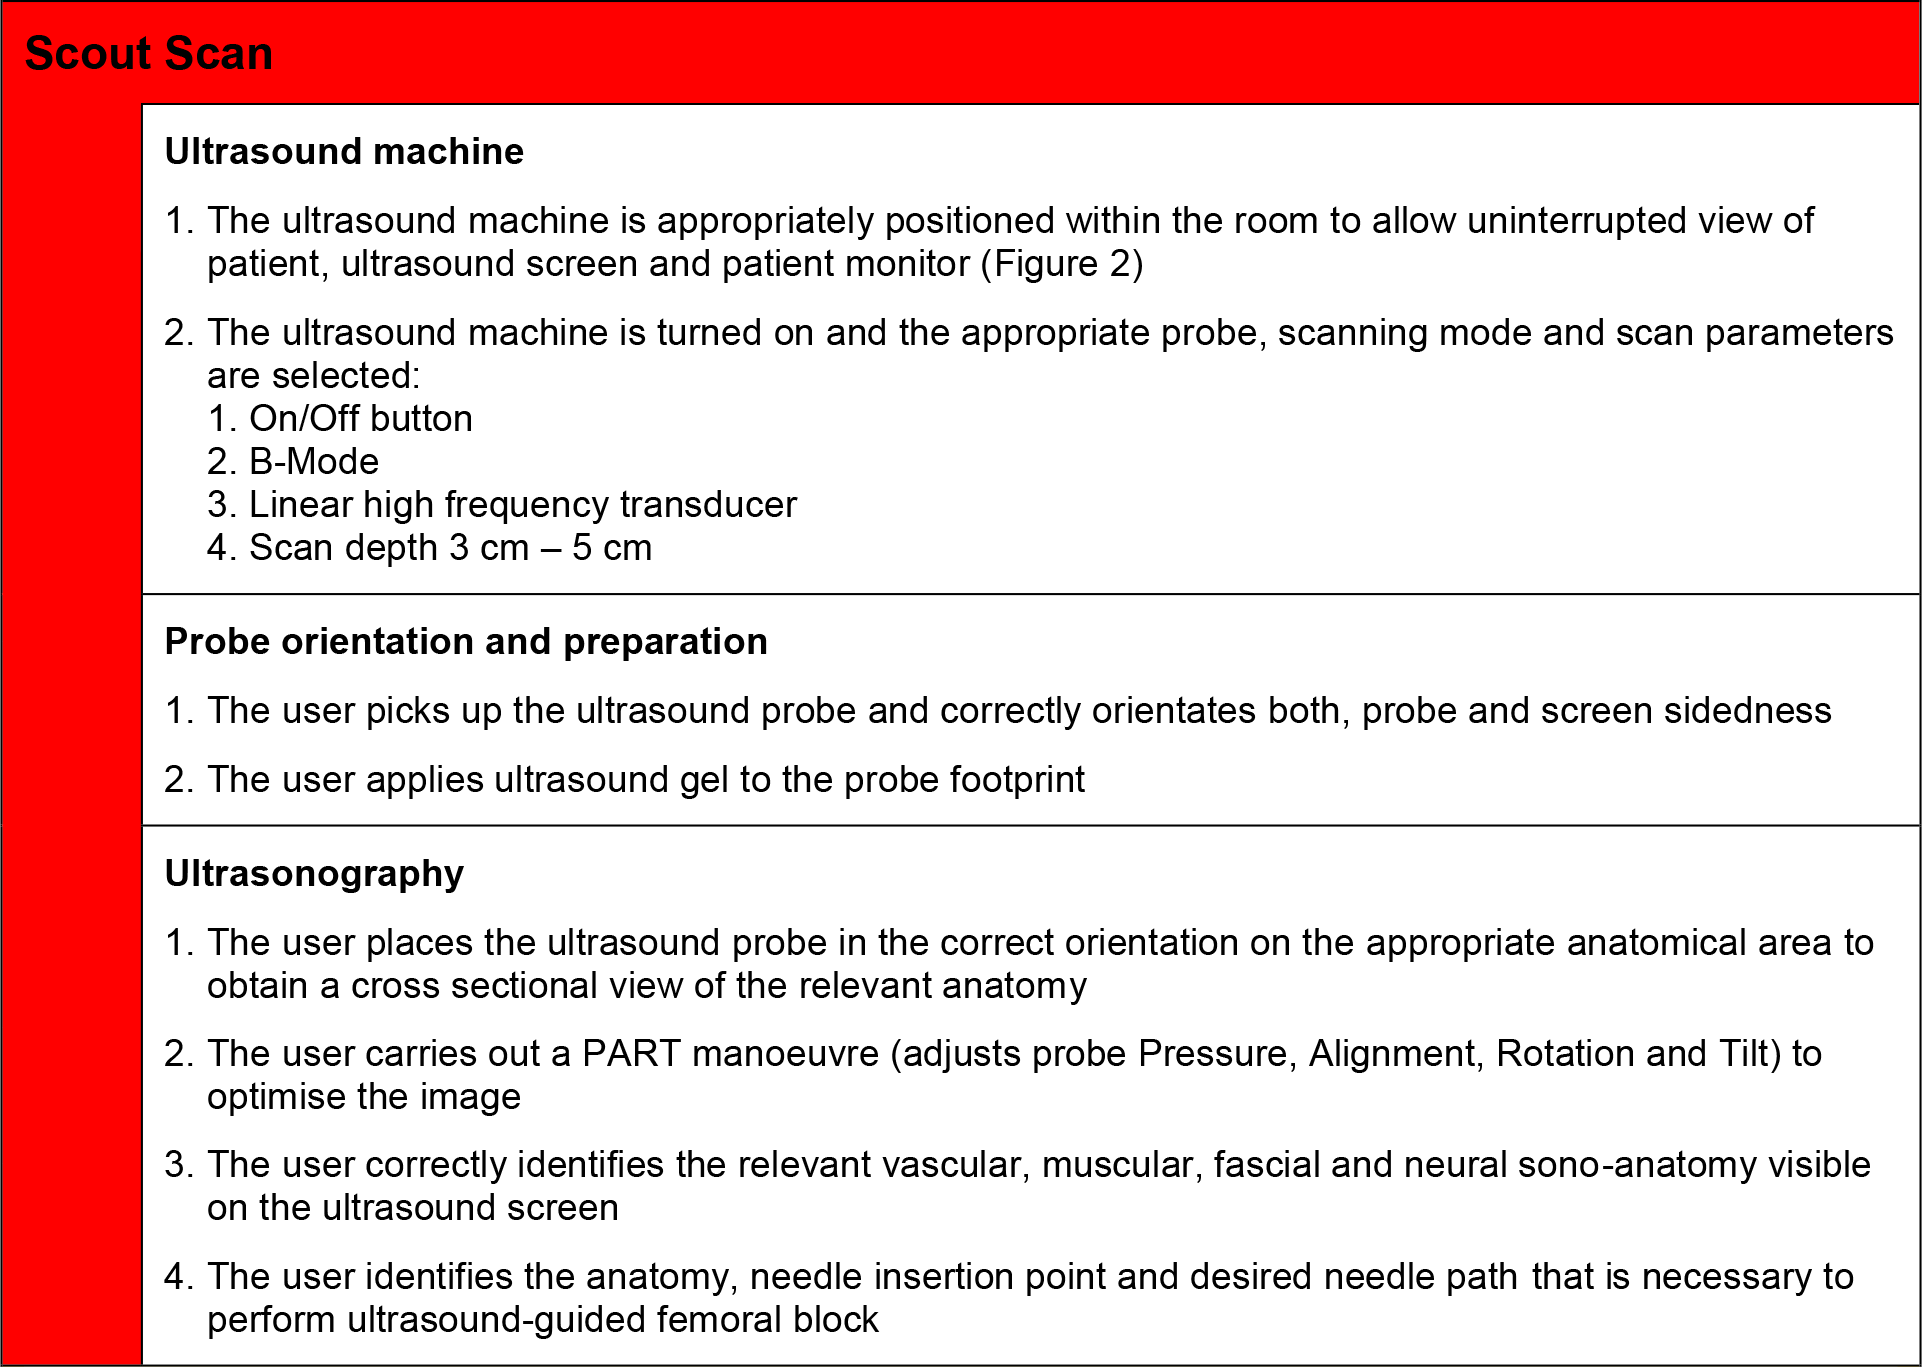
\includegraphics[width=0.8\textwidth]{IMG/scoutscan.png}
    \caption{Tareas del bloque de exploración. }
  \label{fig:scoutscan}
   
\end{figure}
\clearpage
 \begin{figure}[th]
  \centering
    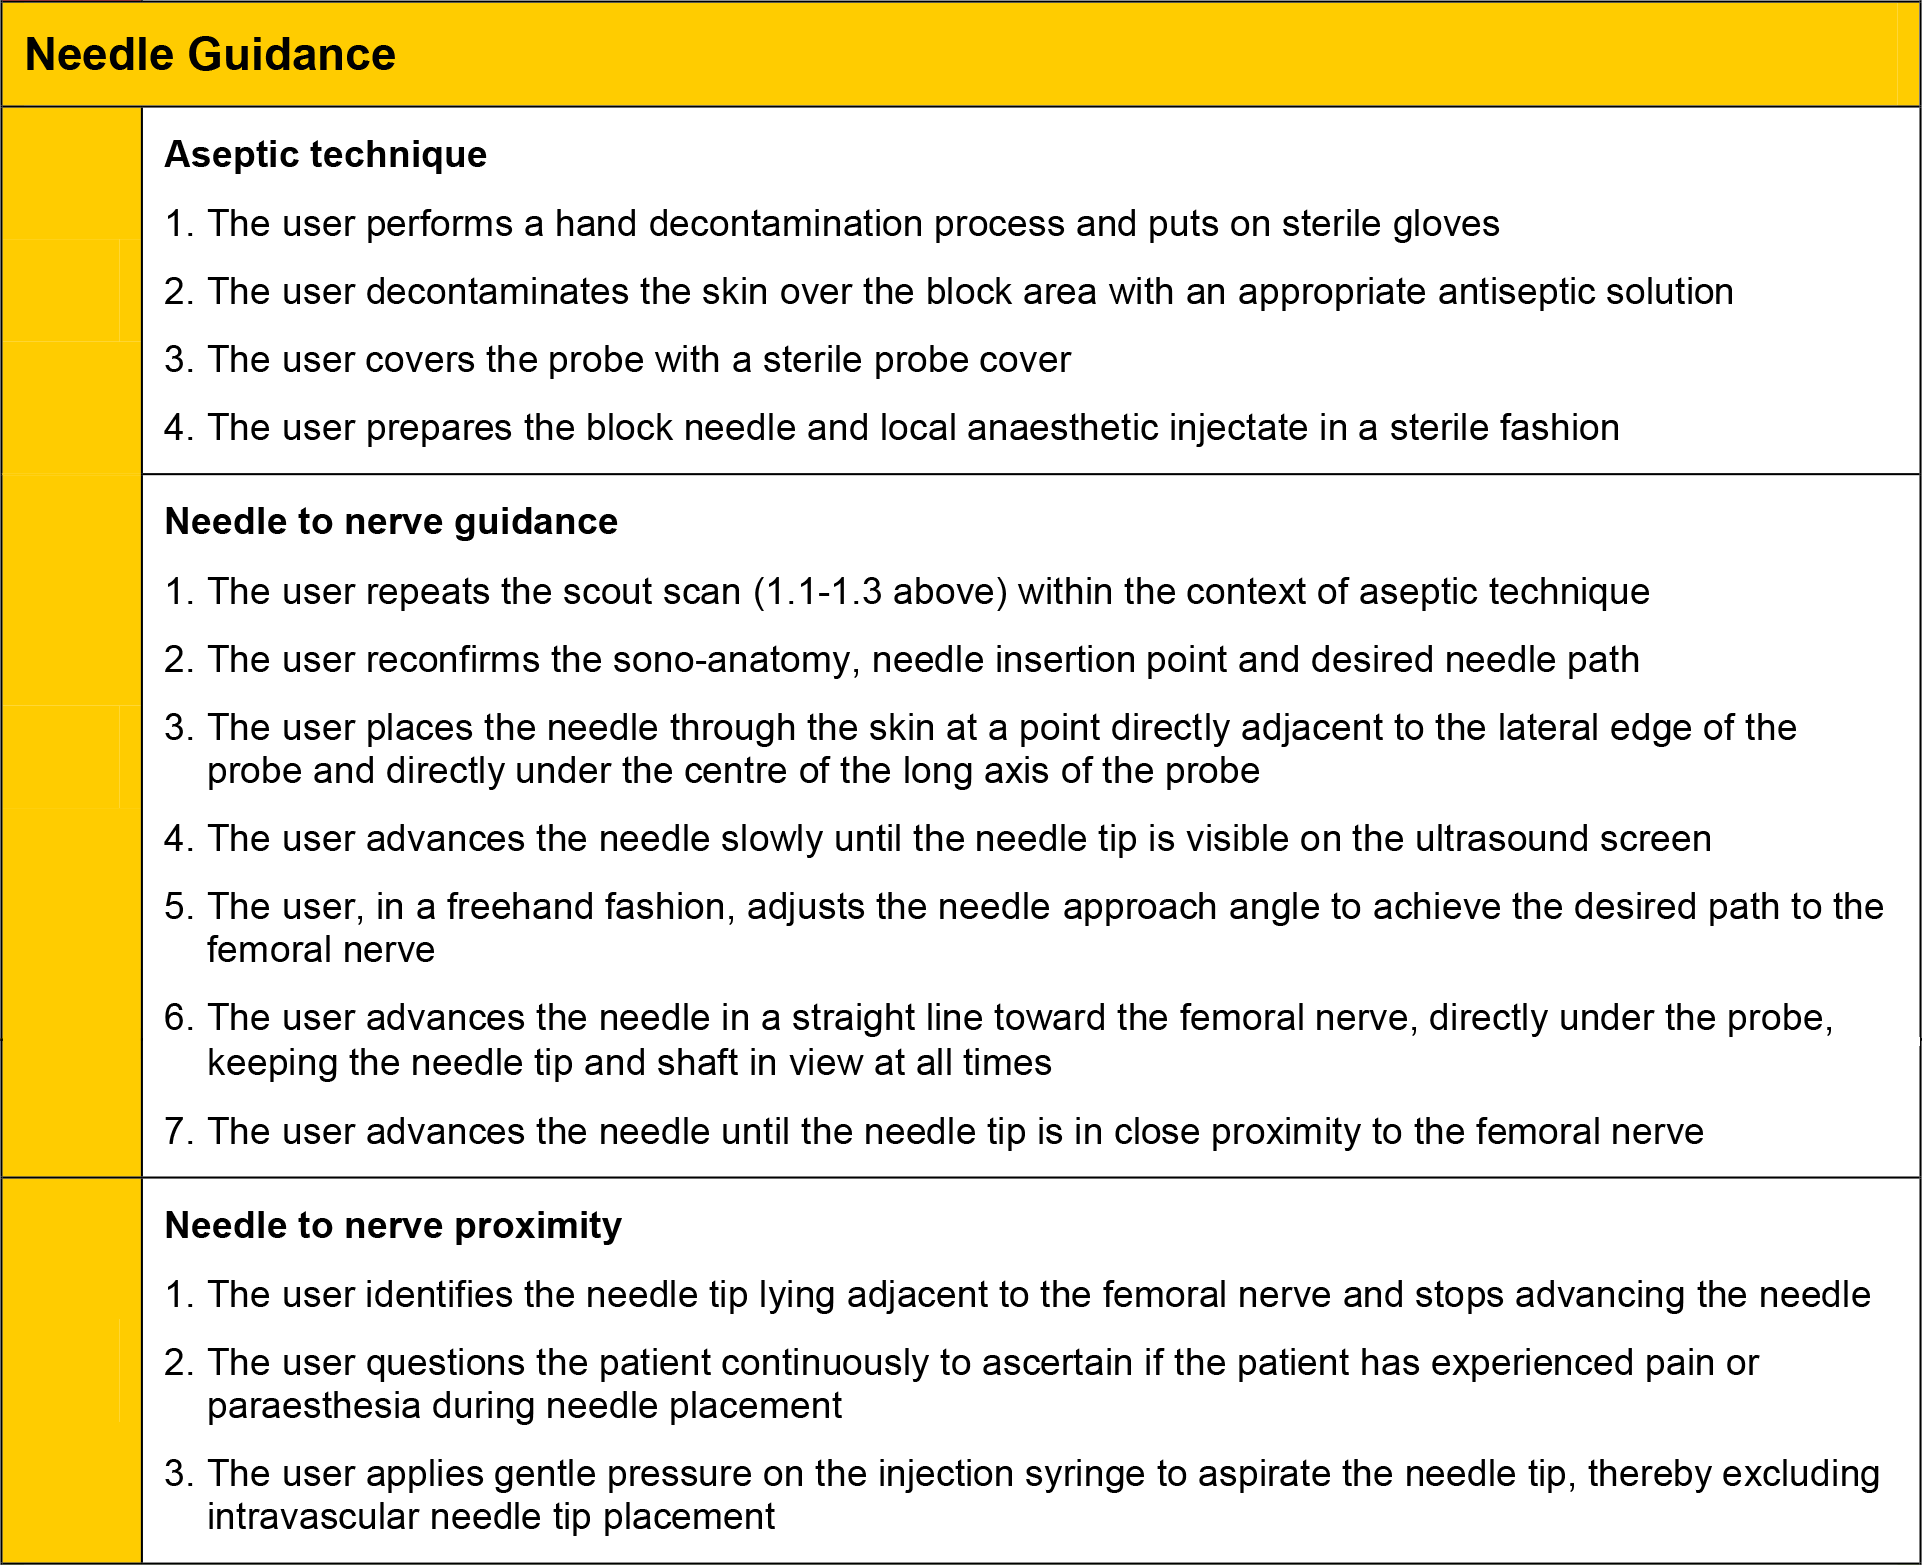
\includegraphics[width=0.8\textwidth]{IMG/needleguidance.png}
    \caption{Tareas del bloque de guiado de la aguja. }
  \label{fig:needleguidance}
\end{figure}
 \begin{figure}[th]
  \centering
    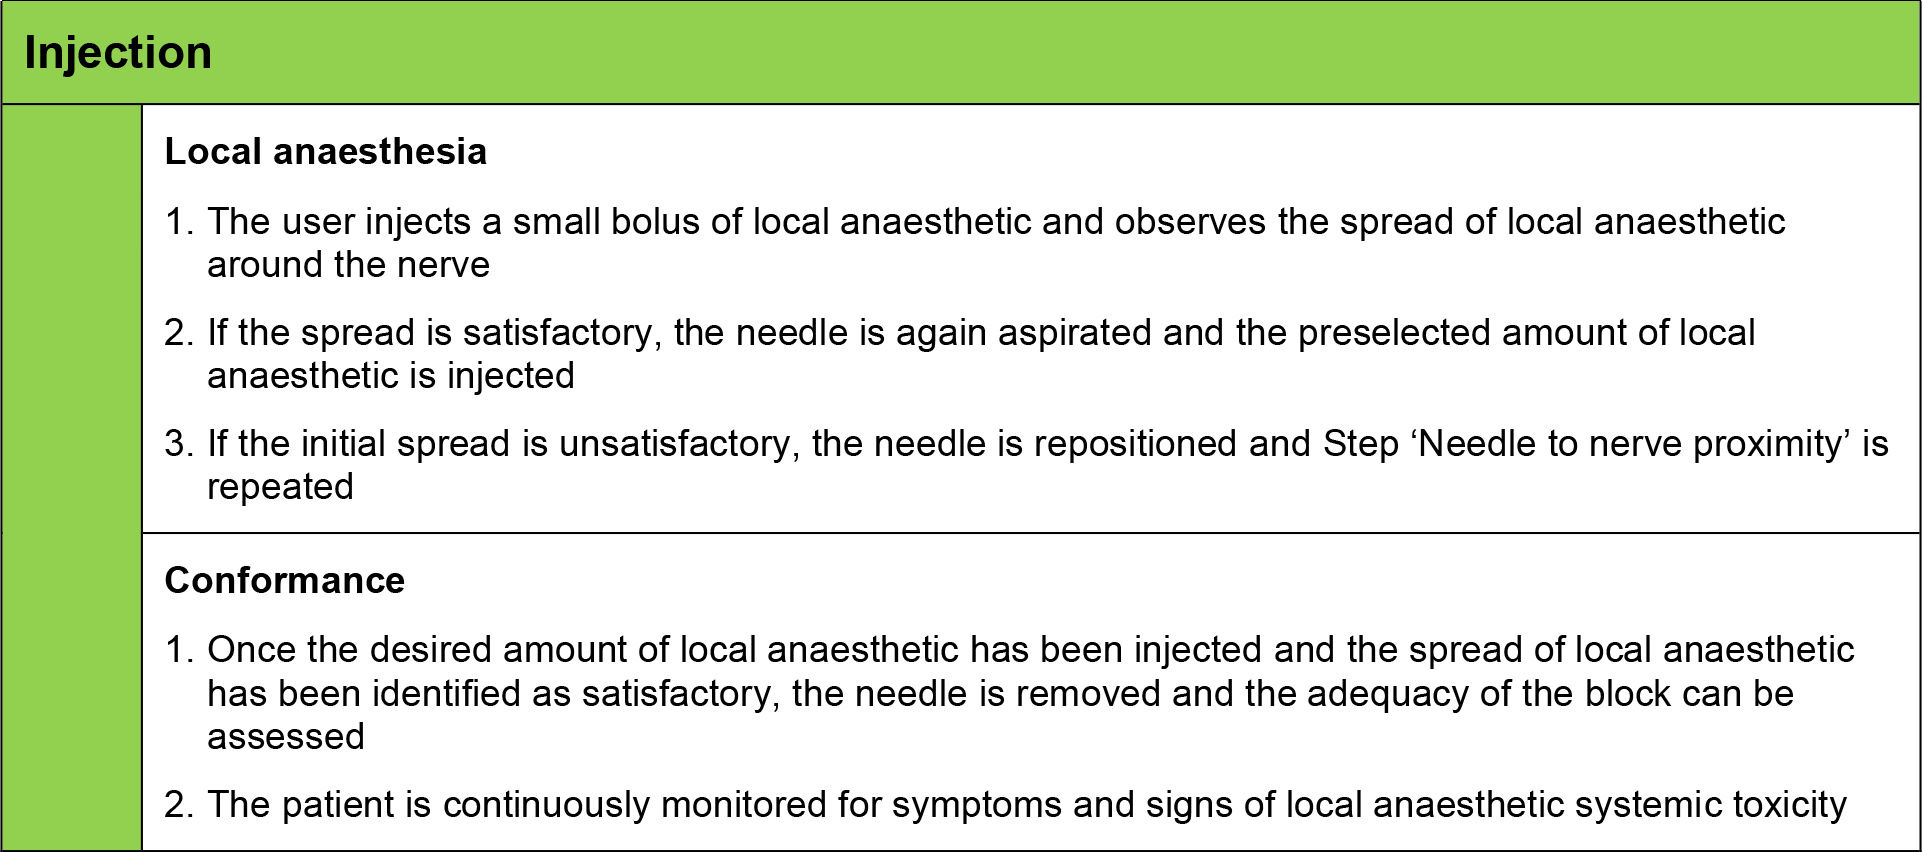
\includegraphics[width=0.8\textwidth]{IMG/injection.png}
    \caption{ Tareas del bloque de inyección.}
  \label{fig:injection}
\end{figure}


% \begin{figure}[h]
%     \begin{subfigure}[b]{0.7\linewidth}
%         \centering
%         {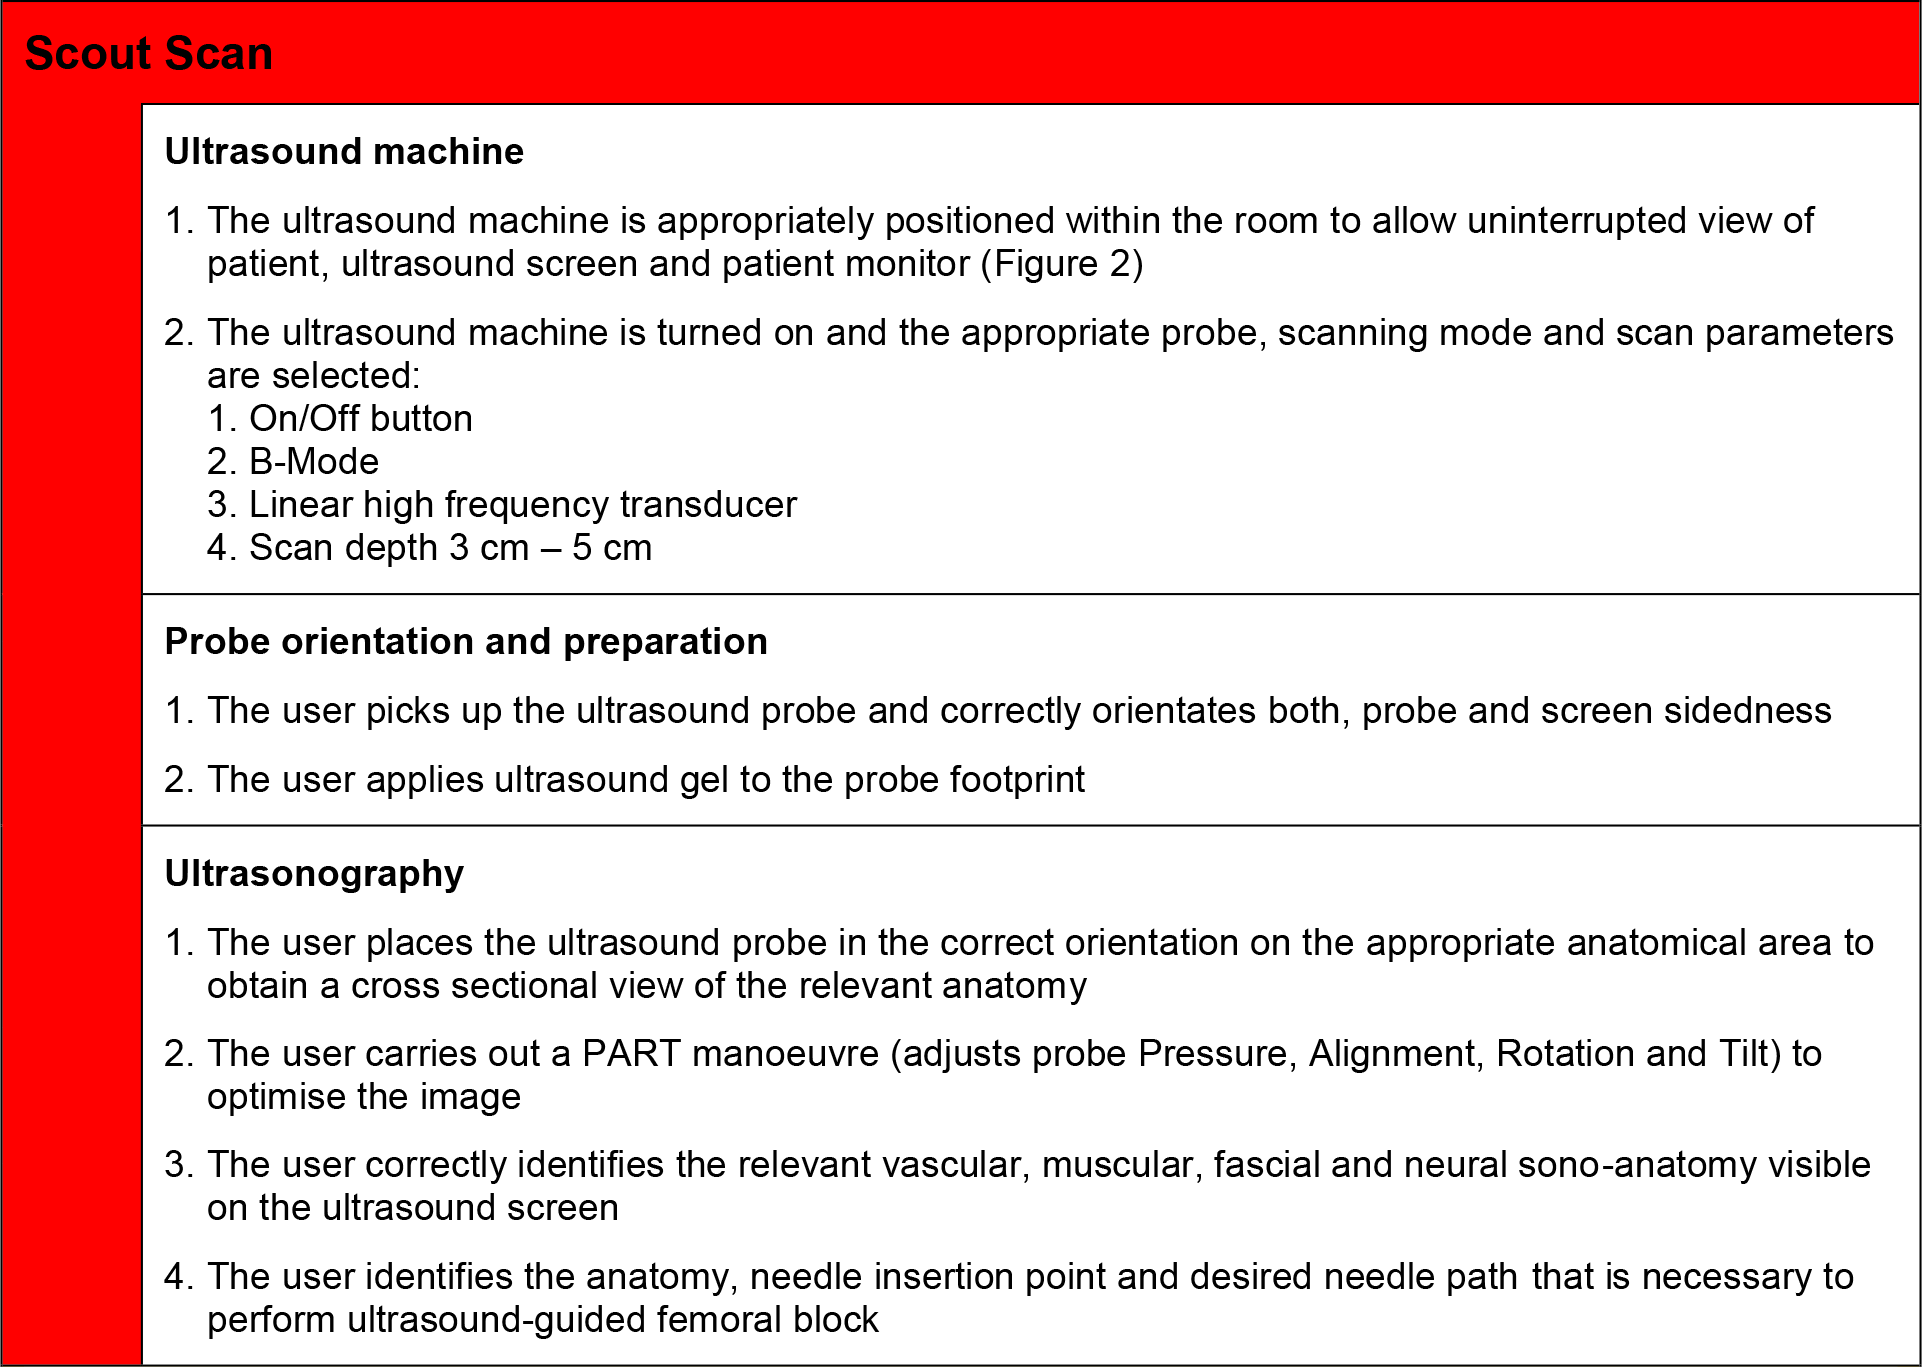
\includegraphics[width=\linewidth]{IMG/scoutscan.png}}
%         \caption{Tareas del bloque de exploración 
%   \label{fig:scoutscan}}
%     \end{subfigure}
%      \begin{subfigure}[b]{0.7\linewidth}
%         \centering
%         {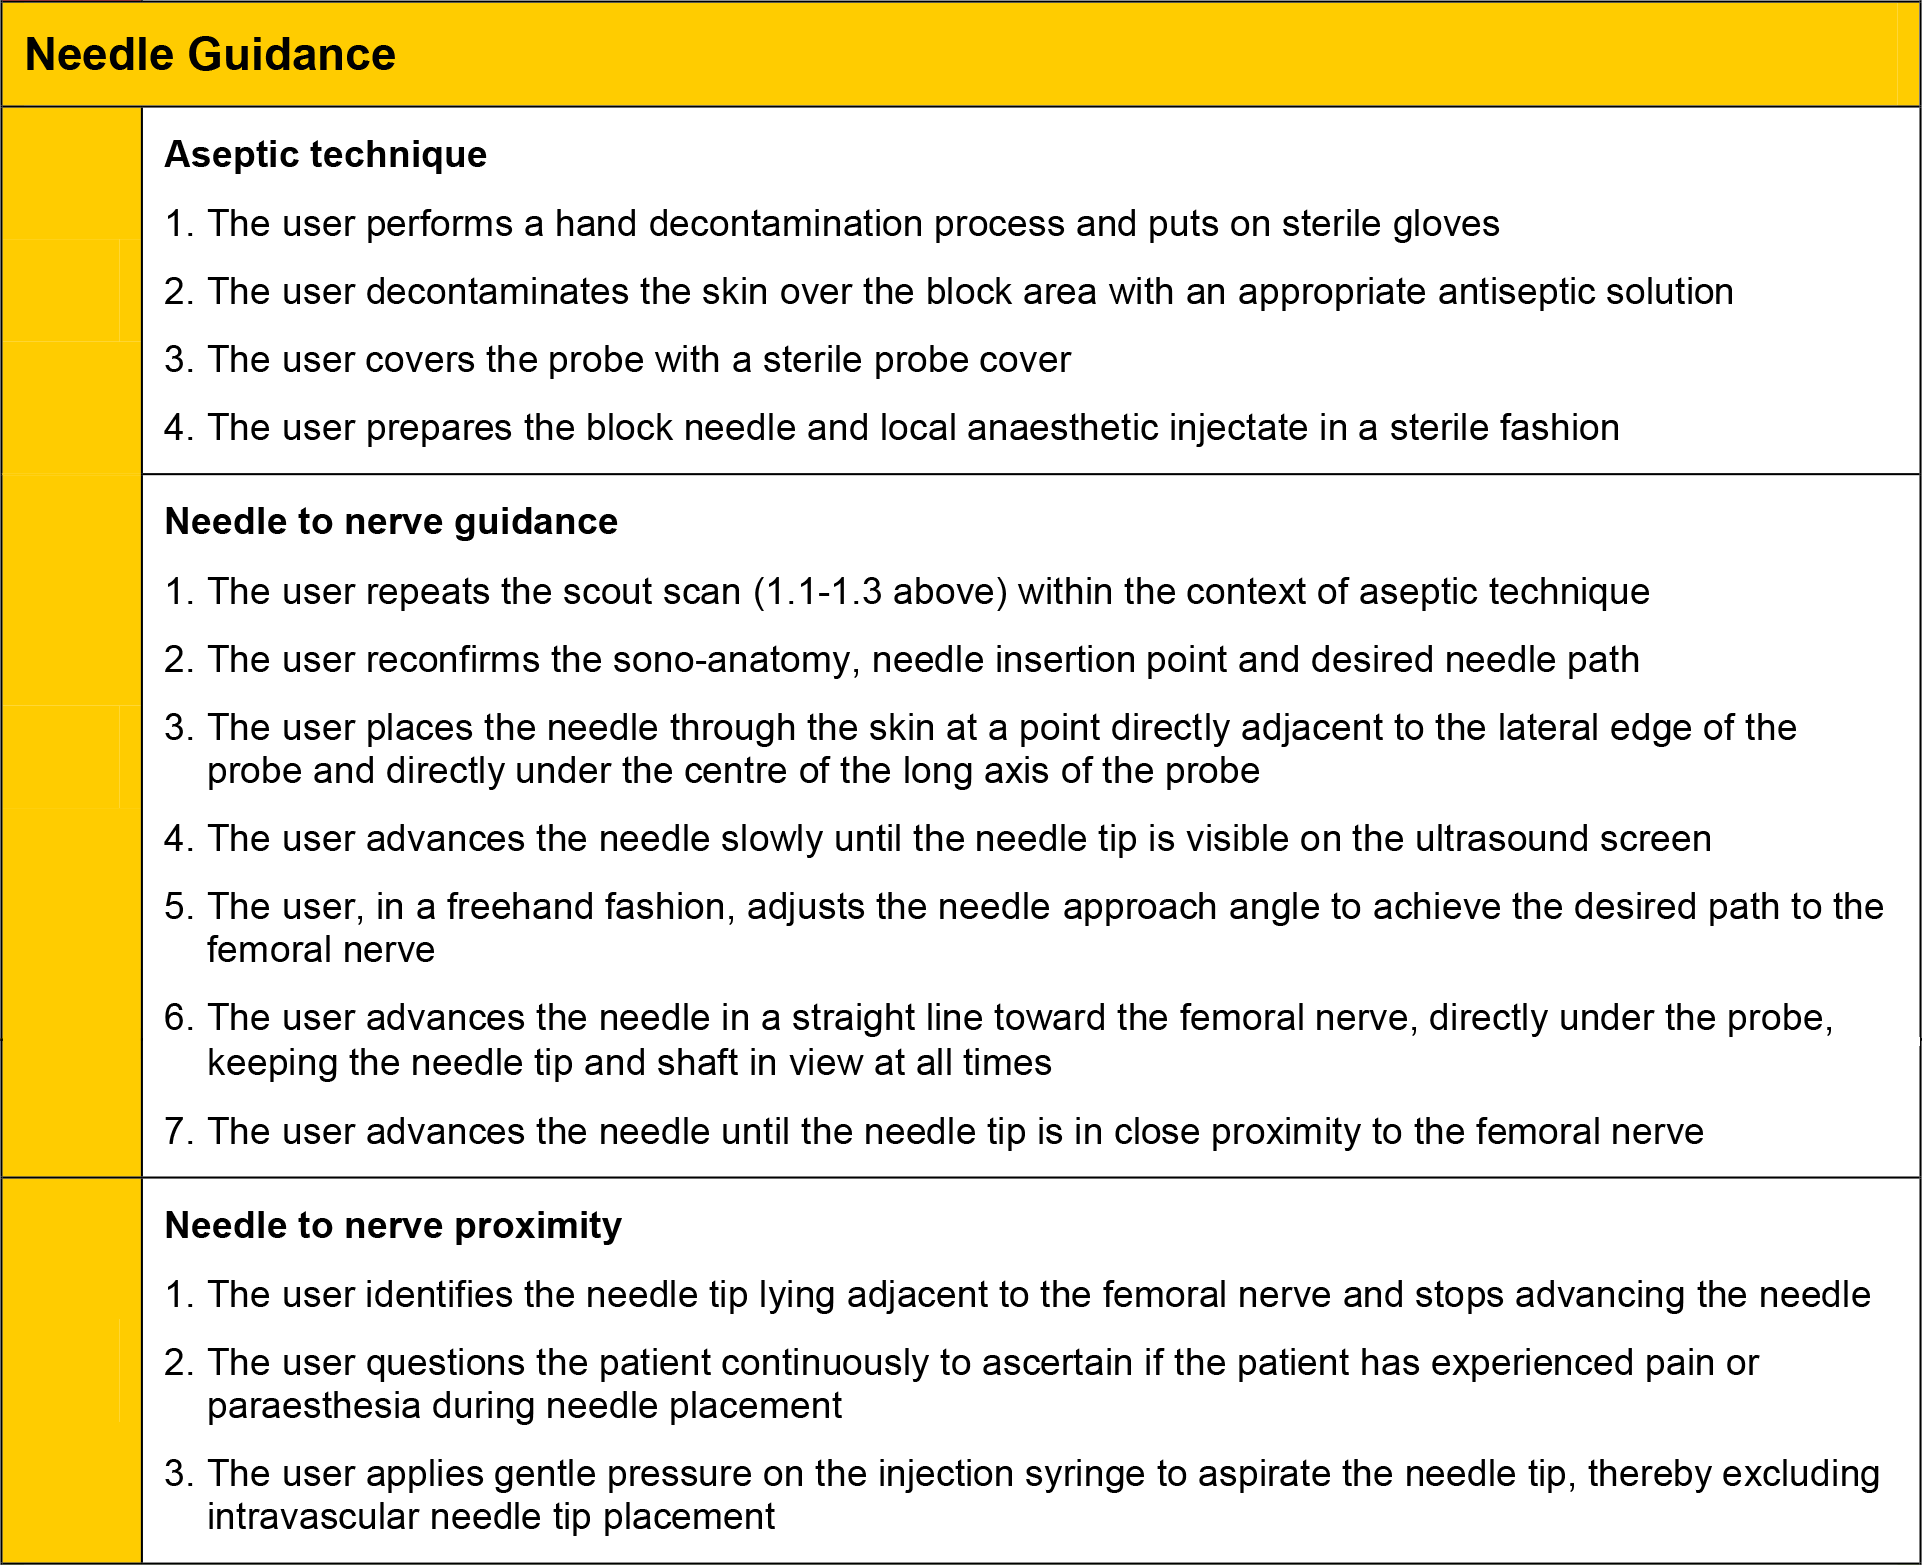
\includegraphics[width=\linewidth]{IMG/needleguidance.png}}
%         \caption{Tareas del bloque de guiado de la aguja. \label{fig:needleguidance}}
%     \end{subfigure}
%      \begin{subfigure}[b]{0.7\linewidth}
%         \centering
%         {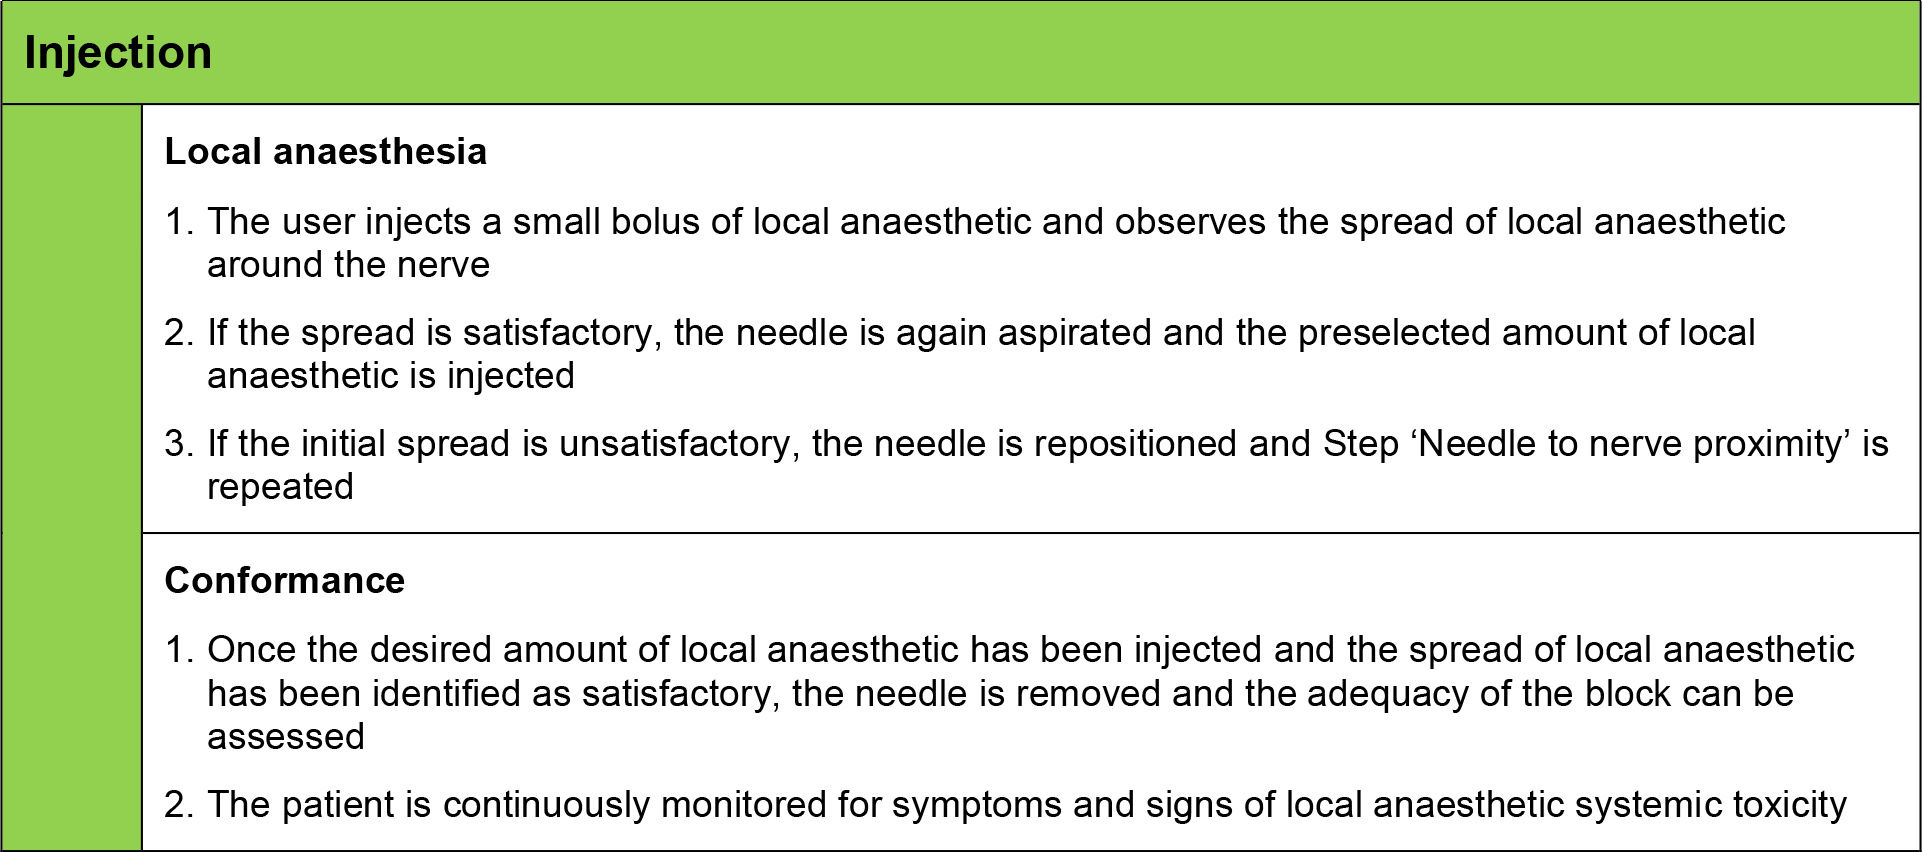
\includegraphics[width=\linewidth]{IMG/injection.png}}
%         \caption{Tareas del bloque de inyección. \label{fig:injection}
%   }
%     \end{subfigure}
%     \caption{Listado del procedimiento completo}
%   \end{figure}
% \clearpage
Con el objetivo de explicar detalladamente cada bloque, se resumirá a continuación el procedimiento completo para un bloqueo femoral:
%
el anestesista deberá posicionarse en la sala de tal forma que su ángulo de visión permita observar al paciente y al monitor de \ac{US} %y al monitor de las constantes vitales
sin mover la cabeza (figura \ref{fig:roomplace}). El médico configurará el equipo de \ac{US} con los valores apropiados y explorará la zona anatómica con la sonda. Para conseguir una imagen adecuada %para identificar los tejidos
, se procederá a la maniobra PART (del inglés \emph{Pressure, Alignment, Rotation and Tilt}) que permite colocar correctamente la sonda de \ac{US} para asegurar una buena imagen donde se puedan localizar todas las estructuras anatómicas relevantes. Una vez el nervio esté localizado, el médico introducirá la aguja en plano\footnote{La aguja se introduce en paralelo con la proyección ultrasonográfica para que quede totalmente visible en la imagen.} con la sonda de \ac{US}, permitiendo así su visualización en la imagen y la dirigirá hasta la proximidad del nervio. Es entonces cuando antes de inyectar el bolo, deberá aspirar primero para comprobar que la punta de la aguja no se encuentre dentro de un vaso sanguíneo y pueda causar toxicidad sistémica \footnote{El anestésico se distribuirá por los vasos sanguíneos.}. Una vez comprobado, a continuación, solo se distribuirá una pequeña cantidad para asegurarse de la localización de la aguja y por último se liberará el bolo completamente. El profesional deberá confirmar que el bloqueo ha sido satisfactorio y comprobará cualquier síntoma de malestar en el paciente.


\begin{figure}[th]
   \centering
    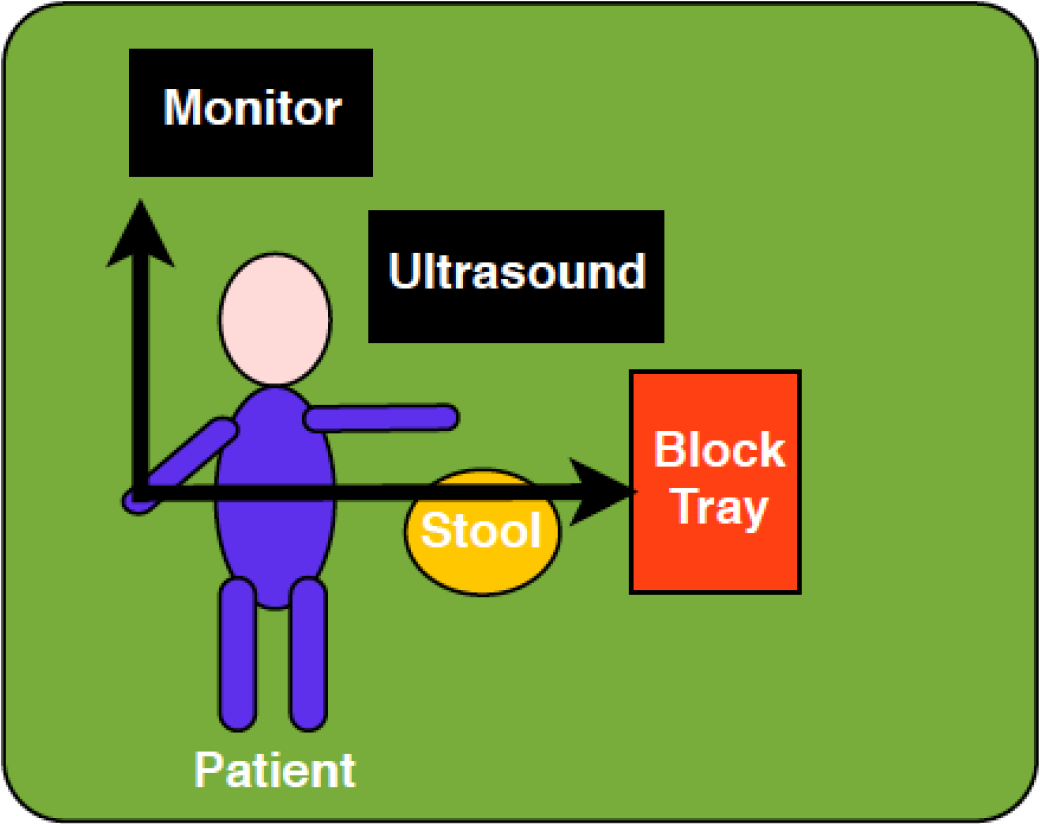
\includegraphics[width=0.5\textwidth]{IMG/roomplacement.png}
    \caption{Diagrama que muestra la disposición del anestesista en la sala de operaciones en un bloqueo femoral. Este se sienta adyacente al paciente, mirando hacia los monitores y con la bandeja de los instrumentos a su derecha.}
   \label{fig:roomplace}
\end{figure}





%https://www.gtsimulators.com/Full-Body-X-Ray-Phantom-with-Real-Human-Skeleton-p/ez7200.htm




% El proyecto \ac{RASimAs} tiene como objetivo  facilitar el entrenamiento y la práctica de la \ac{RA} con la ayuda de un simulador (\ac{RASim}).
% Para que sea utilizado en el mayor número de sitios posibles (hospitales, universidades y colegios profesionales) se debe proporcionar una herramienta de entrenamiento que sea barata, fácil de usar, robusta y que necesite poco mantenimiento.
% Estas herramientas están dirigidas para diferentes perfiles de usuarios.  Tanto estudiantes como profesionales que están empezando a realizar el procedimiento, el simulador les proporcionará un método de entrenamiento con el que mejorar sus habilidades cognitivas y propioceptivas. A su vez, este proyecto también está orientado para profesionales anestesistas que han estado alejados de la práctica del procedimiento y quieran retomar la actividad.
% Los objetivos principales del simulador \ac{RASim} son los siguientes:
% \begin{enumerate}
%     \item El estudiante puede adquirir y desarrollar las habilidades cognitivas y no cognitivas que le permitan ejecutar un bloque de nervio guiado por \ac{US} empezando por el bloqueo del nervio femoral y siguiendo con las siguientes localizaciones.
%     \item Permitir a un anestesista retomar y practicar las habilidades necesarias para realizar el procedimiento de forma segura y satisfactoria.
%     \item Recuperar y medir métricas de rendimiento al realizar el procedimiento en el simulador. 
%     \item Permitir a un supervisor revisar las métricas registradas por los usuarios del simulador a través del tiempo
% \end{enumerate}







%\subsubsection{Objetivos del simulador}


% 6.1.3 Principles of use
% 1. RASim must be contextually relevant and function within the existing or evolving regional
% anaesthesia curriculum
% 2. RASim training must be based upon appropriately detailed characterised procedures
% 3. RASim training must allow the development of relevant procedural skills and associated
% clinical decision making
% 4. RASim training must never allow the development of procedural skill relevant only within
% the simulation environmentRASim training should allow performance related feedback, repeated practice and
% performance tracking and progression over time each based on precisely defined metrics
% 6. RASim based training programmes must have a defined beginning and end (entry and
% exit) constituting proficiency based progression for defined applications e.g. independent
%practice , supervised practice

